\section{Elo Rating System}
The Elo rating system is a method for ranking competitors that is used in Chess and many similar competitor-versus-competitor games. It works by predicting a win-rate of the competitors and then changing the rating according to what the likelihood of the outcome is - if a competitor with a low expected win rate loses, Elo loss is low; however, if that same competitor would win, Elo gain would be very high. Below are the formulae used for our implementation:\\

\noindent The expected winrate of a Script $A$ against a Script $B$ is \\

{\Large\centerline{$E_{A} = \frac{1}{1 + 10^\frac{R_{B}-R_{A}}{400}}$}} \vspace{2mm}

\hspace*{5mm} where $R_{A}$ and $R_{B}$ are the Elo ratings of Script $A$ and Script $B$, respectively.\\

\noindent The resulting rating change of a Script $X$ with an expected winrate $E_{X}$ is \\

{\Large\centerline{$R_{X}' = R_{X} + 32(W - E_{X})$}} \vspace{2mm}

\hspace*{5mm} where $R_{X}$ is the old rating of $X$, $R_{X}'$ is the new updated rating \\
\hspace*{17mm} and $W$ is a value $1$ or $0$ if $X$ wins or loses, respectively.\\

All scripts begin with an $R_{X}$ of 1400.  For games with more than two racers, each racer `wins' against anyone they finish ahead of, and `loses' to anyone they finish behind. $E_{X}$ is calculated against each script. For example, in a 3-way race, the 2\textsuperscript{nd} place finisher loses Elo as if it had lost a head-to-head race with the 1\textsuperscript{st} place script, but gains Elo as if it had defeated the 3\textsuperscript{rd} place script in a head-to-head. Depending on the ratings of the scripts at the start of the race, this script could have a net positive or negative Elo change.
\section{Instruction Manual (Handout)}

\begin{figure}[H]
\centering
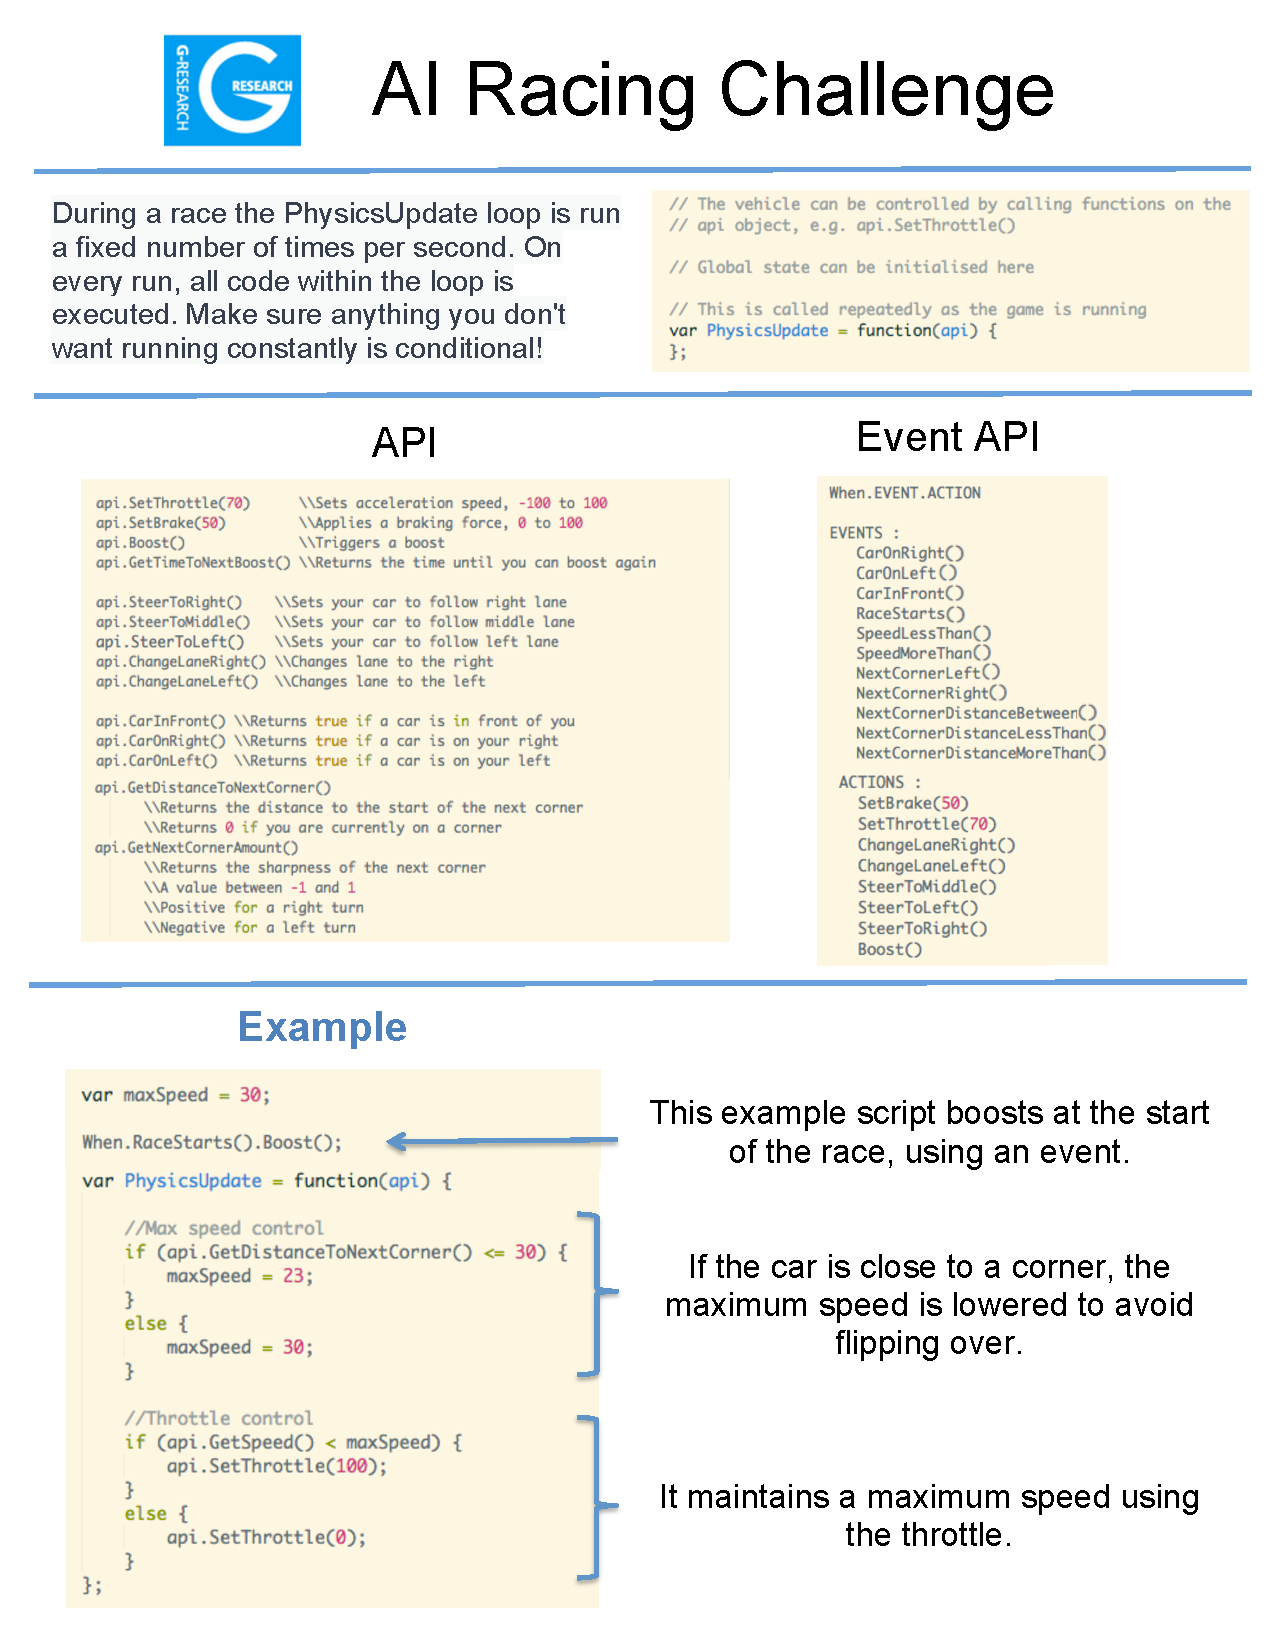
\includegraphics[width=\textwidth,page=1]{Handout.pdf}
\caption{Handout - first page.}
\end{figure}
\begin{figure}[H]
\centering
\includegraphics[width=\textwidth,page=2]{Handout.pdf}
\caption{Handout - second page.}
\end{figure}

\section{Development Process}

\begin{figure}[H]
\centering
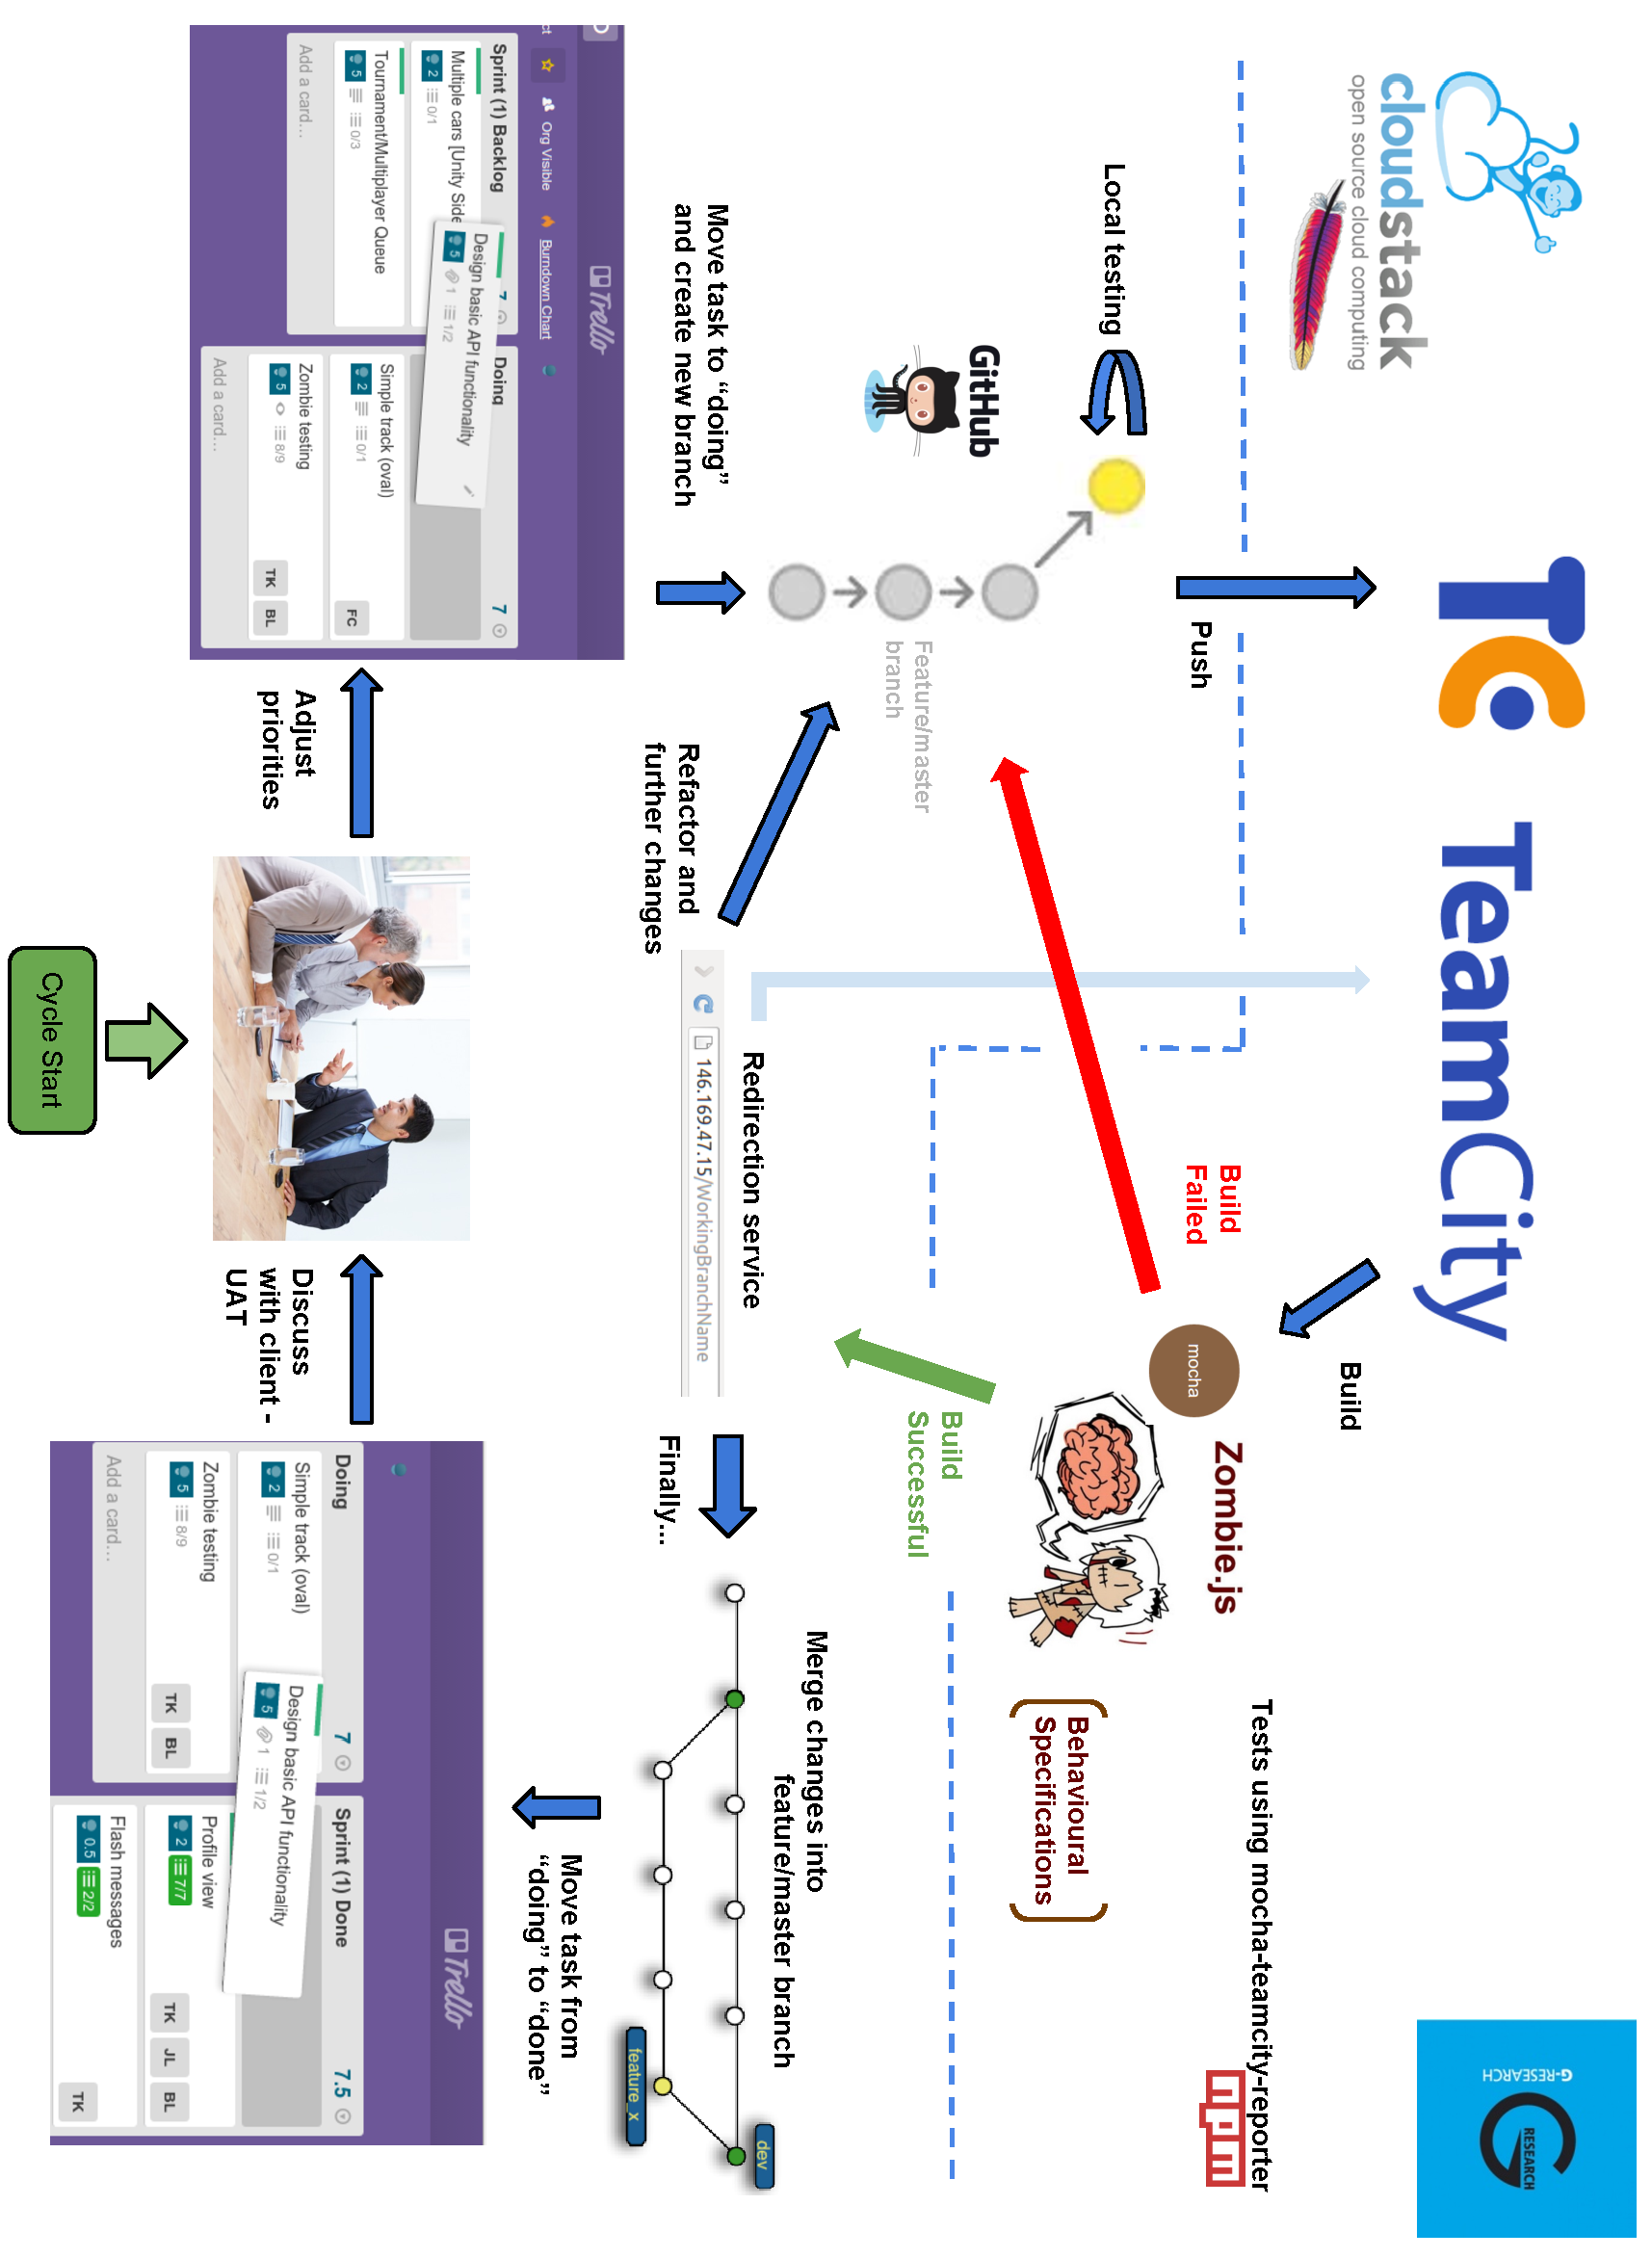
\includegraphics[width=\textwidth]{DevProcess.pdf}
\caption{Development process diagram.}
\end{figure}